\subsection{Visual-Question Answering}
\label{sec:vqa}
The \textit{Visual-Question Answering} (VQA) problem refers to the ability of a system of ``reasoning'' over an image, based on a given query expressed in terms of text. This means that, given in input an arbitrary image and an arbitraty textual prompt the system must be able to generate an answer to the given prompt (Figure \ref{fig:vqa_example}).
\begin{figure}[t]
    \centering
    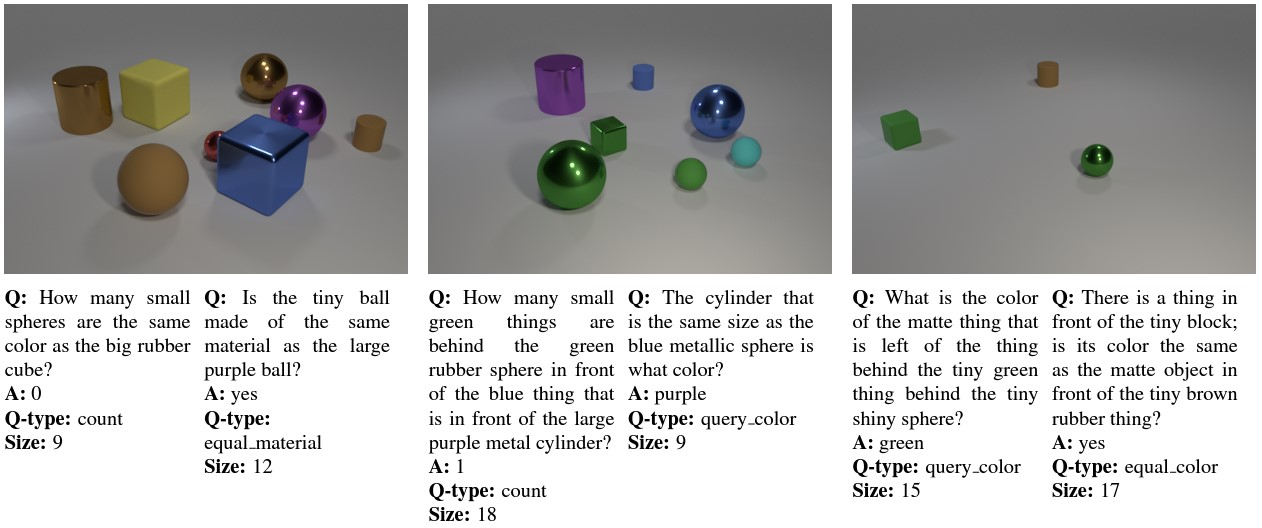
\includegraphics[width=1.0\textwidth]{figures/images/ch2/vqa_problem.jpg}
    \caption{Example of Vision-Question Answering problem get from the CLEVR \cite{johnson2017clevr} dataset. It is possible to observe how for a given image multiple different questions can be done. As well as, questions covers different reasoning skills such as attribute identification, counting, comparison, multiple attention, and logical operations.}
    \label{fig:vqa_example}
\end{figure}


The key aspect related to this problem is related to the fact that for a given image different questions can be made, this means that there is not an a priori mapping between the input image and the corresponding answer, but the system must be able to dynamically adapt its \textbf{attention} on specific part of the image based on the given query, meaning that the system must be able to correlate in an effective way the encoding of the image and the encoding of the prompt, in order to create a \textbf{conditioned} embedding that can be effectively used to generate a valid answer.

Based on these preliminary considerations, various solutions have been proposed using both Convolutional Neural Network architectures \cite{perez2018film} and novel Transformer architectures \cite{chen2022caan,chen2024mpcct,liu2024visual}.

A significant breakthrough in this field was introduced in \cite{perez2018film}, where the FiLM (Feature-wise Linear Modulation) conditioning layer was proposed. The core idea behind FiLM is to adaptively modify the output of a neural network by applying an affine transformation to its intermediate features based on some input. Specifically, the FiLM layer learns two functions, $f$ and $h$, which produce the coefficients $\gamma_{i,c}$ and $\beta_{i,c}$, respectively, based on an input $x_{i}$, as defined in Equation \ref{eq:film}.
\begin{equation}
    \label{eq:film}
    \begin{matrix}
        \gamma_{i,c} = f_{c}(x_{i}) & 
        \beta_{i,c} = h_{c}(x_{i})
    \end{matrix}
\end{equation}
These coefficients are then used to modulate the $c^{th}$ activation map $\textbf{F}_{i,c}$ through a \textit{feature-wise affine transformation}, as described in Equation \ref{eq:film_eq}.
\begin{equation}
    \label{eq:film_eq}
    FiLM(\textbf{F}_{c}|\gamma_{c}, \beta_{c}) = \gamma_{c} \textbf{F}_{c} + \beta_{c}
\end{equation}

An example of integrating the FiLM layer into a deep architecture is shown in Figure \ref{fig:film_architecture}, illustrating the implementation proposed in \cite{perez2018film}. In this configuration, the prompt is encoded using a Gated Recurrent Unit (GRU), and the resulting embedding is fed into a Multi-Layer Perceptron (MLP), which outputs the coefficients $\gamma_{i,c}$ and $\beta_{i,c}$. These coefficients are subsequently used to modulate the activations of $N$ Residual Blocks (ResBlocks).
\begin{figure}[t]
    \centering
    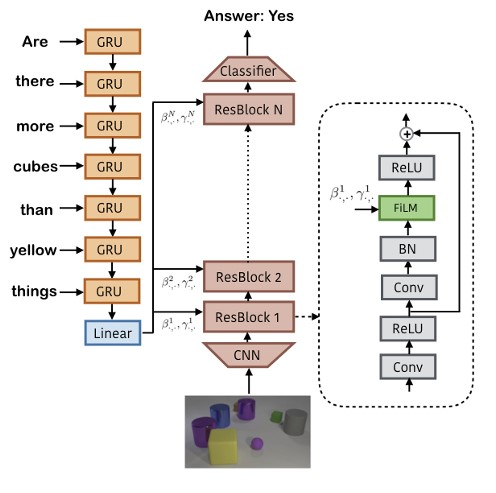
\includegraphics[width=0.6\textwidth]{figures/images/ch2/film_architecture.jpg}
    \caption{Proposed integration of the FiLM conditioning layer. Here, the Linear Modulation is applied to modify the activation maps of the ResNet blocks, while a linear layer generates the modulation coefficients $\beta$ and $\gamma$ based on the embedding derived from the textual prompt. This enables the model to conditionally adjust the activation maps according to the context provided by the input query}
    \label{fig:film_architecture}
\end{figure}


The FiLM layer has also been effectively applied in the context of Language-Conditioned Policy Learning (Section \ref{sec:occp_mtil}) \cite{jang2022bc_z,brohan2022rt}. Starting from a textual prompt describing a desired task, the FiLM layer modulates the activation maps of the convolutional blocks in the network that encodes the robot's observations. This allows the network to focus on specific parts of the image relevant to the task (Figure \ref{fig:film_attention}).
\begin{figure}[t]
    \centering
    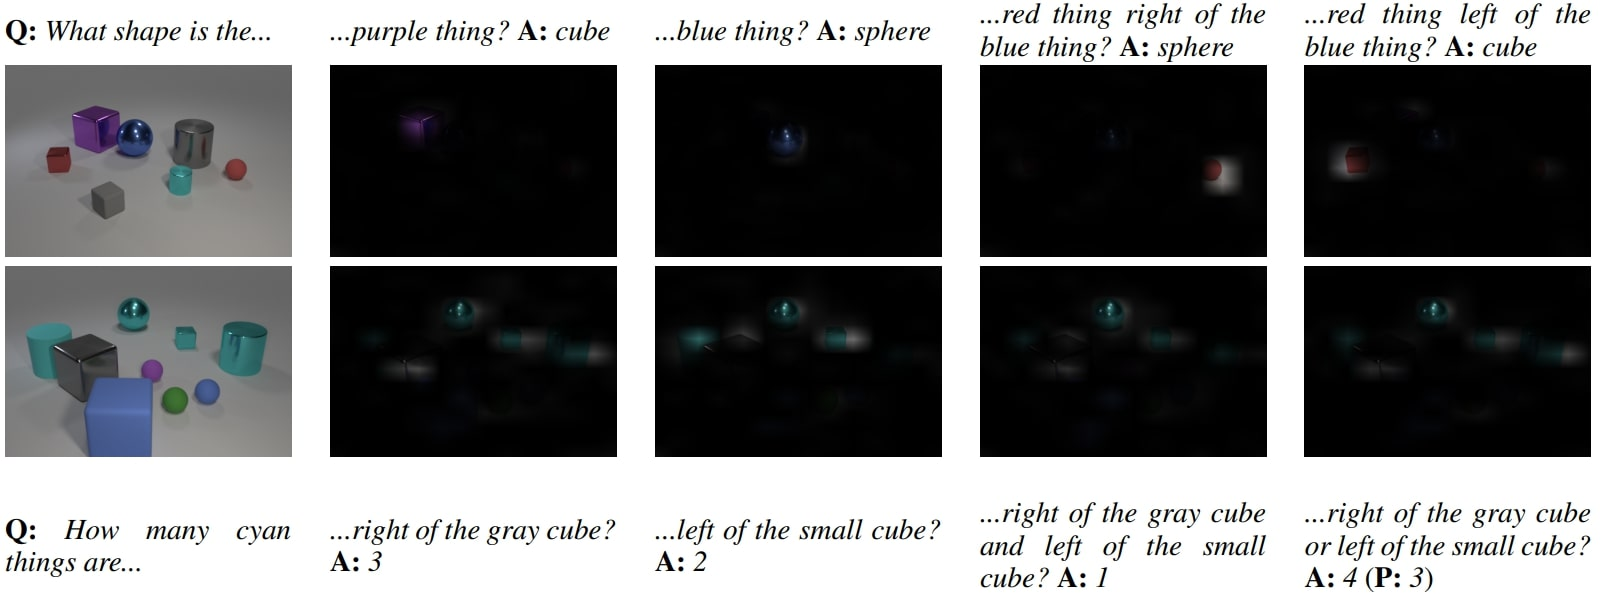
\includegraphics[width=0.9\textwidth]{figures/images/film/film_attention.jpg}
    \caption{Visualizations of the distribution of locations used by the model for its globally max-pooled features, from which its final MLP makes predictions. FiLM correctly localizes the object referenced by the answer (top) or all objects referenced by the question (bottom). However, the localization is less accurate when the model provides an incorrect answer (rightmost bottom).}
    \label{fig:film_attention}
\end{figure}


Since the introduction and expansion of Transformer models \cite{vaswani2017attention}, there has been a major shift towards solving the Visual Question Answering (VQA) problem by utilizing these architectures. Transformers excel at capturing intra-modal relationships through dependency modeling and promoting alignment and interaction between multiple modalities. This has led to the development of Vision-Language Transformers capable of directly processing multi-modal inputs, such as images and text. An example is the LLaVA model proposed in \cite{liu2024visual}, which represents the current state-of-the-art in VQA. However, despite its capability to handle complex queries, LLaVA relies on a Large Language Model (LLM) with a minimum size of 7 billion parameters, requiring a high-performance server. This makes real-time deployment in real-world systems, such as robotic control, challenging or even impractical.
